\clearpage\section{Statement of the Problem and Specific Aims}\label{intro}

Statement of the problem and specific aims of the overall project.

\begin{figure}[p]
  \begin{subfigure}{\textwidth}
    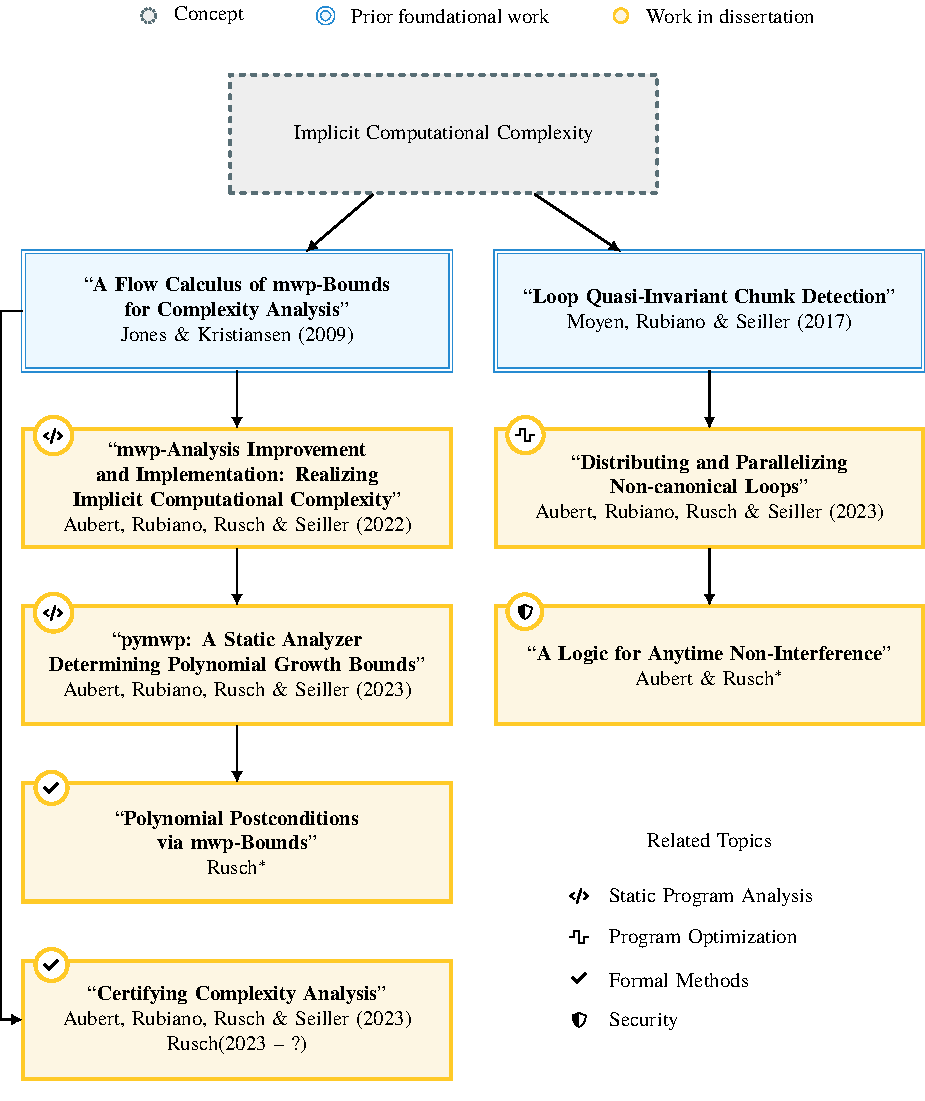
\includegraphics[width=\linewidth,keepaspectratio]{fig_conn_papers}
  \end{subfigure}
  \begin{center}
  \resizebox{.85\textwidth}{!}{
  \begin{subfigure}{\textwidth}{
    \begin{tabularx}{\textwidth}{@{}X@{}cr@{}}
      \toprule
      \textbf{Title} & \textbf{Section} & \textbf{Background} \\
      \midrule
      {mwp-Analysis Improvement and Implementation\ldots}
      & \aref{sec:fscd}
      & \ref{icc}, \ref{static-analysis}, \ref{flow-calculus} \\
      {Distributing and Parallelizing Non-canonical Loops}
      & \ref{sec:vmcai}
      & \ref{transforms} \\
      {Polynomial Postconditions via mwp-Bounds}
      & \ref{sec:postcond}
      & \ref{flow-calculus}, \ref{verification} \\
      {pymwp: A Static Analyzer Determining\ldots}
      & \ref{sec:atva}, \aref{app:toolguide}
      & \ref{icc}, \ref{static-analysis}, \ref{flow-calculus} \\
      {A Logic for Anytime Non-Interference}
      & \ref{sec:anytime}
      & \ref{pl-sec} \\
      {Certifying Complexity Analysis}
      & \ref{coqpl}
      & \ref{flow-calculus}, \ref{verification} \\
      \bottomrule
    \end{tabularx}}
  \end{subfigure}}
  \end{center}
  \caption[Connected papers]{Connections between dissertation publications.}
  \label{fig:conn_papers}
\end{figure}

% How to read notes
%
% All PDF files referenced in this dissertation are archived on Internet Archive.
% To recover a URL from the archive:
% https://web.archive.org/web/<URL>
% For example,
% https://web.archive.org/web/https://types22.inria.fr/files/2022/06/TYPES_2022_paper_14.pdf
% produces the corresponding document.
%
% TODO: Software notes

\clearpage\section{Review of the Literature}\label{sec:pre}

Literature review and discussion of the rationale of the project.
It is expected that the literature review will be more comprehensive than
those presented in the included publications.

\begin{lstlisting}[style=Dafny,caption={a code block test}]
/* long comment */
method DafnyEx() {
  var x := 100;
  while x > 0 {
    x := x - 1;
  }
  assert x == 0;
}
\end{lstlisting}


\subsection{Literature Topic 1: Implicit Computational Complexity}\label{icc}
\subsection{Literature Topic 2: Static Resource Analysis}\label{static-analysis}
\subsection{Literature Topic 3: The Flow Calculus of mwp-Bounds}\label{flow-calculus}
\subsection{Literature Topic 4: Formal Verification}\label{verification}
\subsection{Literature Topic 5: Loop Transformations for Parallel Programming}\label{transforms}
\subsection{Literature Topic 6: Confidentiality and Non-Interference}\label{pl-sec}